\documentclass[a4paper,12pt]{article}
\usepackage[utf8]{inputenc}
\usepackage{amsmath, amssymb, amsthm, graphicx, pgfplots, tikz}
\usepackage{lmodern} 
\usepackage[german]{babel}  
\usepackage{csquotes} 


\pgfplotsset{compat=1.18}

\newtheorem{theorem}{Theorem}[section]
\newtheorem{lemma}[theorem]{Lemma}
\newtheorem{corollary}[theorem]{Korollar}


\theoremstyle{definition}
\newtheorem{definition}[theorem]{Definition}

\theoremstyle{remark}
\newtheorem*{remark}{Bemerkung}

\title{Fourier-Methoden: Theorie und Anwendungen}
\author{Felix Wager}
\date{\today}

\begin{document}

\maketitle

\renewcommand{\contentsname}{Inhaltsverzeichnis}
\tableofcontents
\newpage


\section{Abstract}

\section{Einleitung}
\subsection{Motivation}
Warum Fourier-Methoden heute so wichtig sind.
\subsection{Zielsetzung der Arbeit}
\subsection{Aufbau der Arbeit}

\section{Mathematische Grundlagen}
\subsection{Komplexe Zahlen und die Eulerformel}
Um sich die Arbeit mit Fourier Transformationen, Reihen und sonstigem erheblich zu erleichtern ist es sehr sinnvoll mit komplexen Zahlen zu arbeiten. Doch was sind komplexe Zahlen? 
Komplexe Zahlen sind prinzipiell nichts anderes, als eine Erweiterung der Menge der Reellen Zahlen, welche es ermöglicht die Wurzel von negativen Zahlen zu ziehen. Dafür wird die Wurzel die imaginäre Einheit $i$ definiert. Mathematisch korrekt sieht das wie folgt aus:
$$i^2 = -1$$
Die Menge der komplexen Zahlen wird mit dem Symbol $\mathbb{C}$ abgekürzt. Eine typische komplexe Zahl hat in der algebraischen Schreibweise die Form:
$$ z = a + ib \quad \text{mit} \quad a,b \in \mathbb{R} $$
$a$ ist hierbei der Realteil $\Re(z)$ und $b$ der Imaginärteil $\Im(z)$ von $z$. \vspace{1em}

Um mit komplexen Zahlen bei Fourier Reihen zu arbeiten, benötigt man auch ein paar Rechenoperationen. Die wichtigsten beiden sind hier der Betrag und das komplex konjugierte einer komplexen Zahl. Eine komplexe Zahl lässt sich auch als Vektor im $\mathbb{R}^2$ betrachtet, so ist dann der Betrag als euklidische Norm dieses Vektors definiert. 
$$\vert{z}\vert = \sqrt{ a^2 + b^2}$$
Bedeutet in einem Koordinatensystem, bei dem der Real- und Imaginärteil einer Zahl auf den x- und y-Achsen festgehalten wird, ist der Betrag die Länge vom Ursprung bis zum Punkt im Koordinatensystem dieser Zahl. 
Und das komplex konjugierte einer Zahl ist eine Abbildung, welche lediglich den Imaginärteil mit $-1$ multipliziert:

$$\bar{}\;:\mathbb{C}\;\to\mathbb{C},\; z = x+iy \mapsto \bar{z} := x-iy$$

Mithilfe von komplexen Zahlen und den Taylorreihen von Sinus, Cosinus und der Exponentialfunktion $e^x$ kann man nun die Eulerformel herleiten. 

% $$e^{ix} = \cos{x} + i\sin{x}$$

Wenn man den Betrag dieses Ausdrucks bildet, so fällt auf, dass hier das Ergebnis, unabhängig von $x$, 1 ist. Dies bedeutet, dass $e^{ix}$ als ein gegen den Uhrzeigersinn rotierender Vektor, für steigende Werte für $x$, gesehen werden kann. Im vorher genannten Koordinatensystem, welches man auch die Gaußsche Zahlenebene nennt, sieht das so aus:
\begin{center}
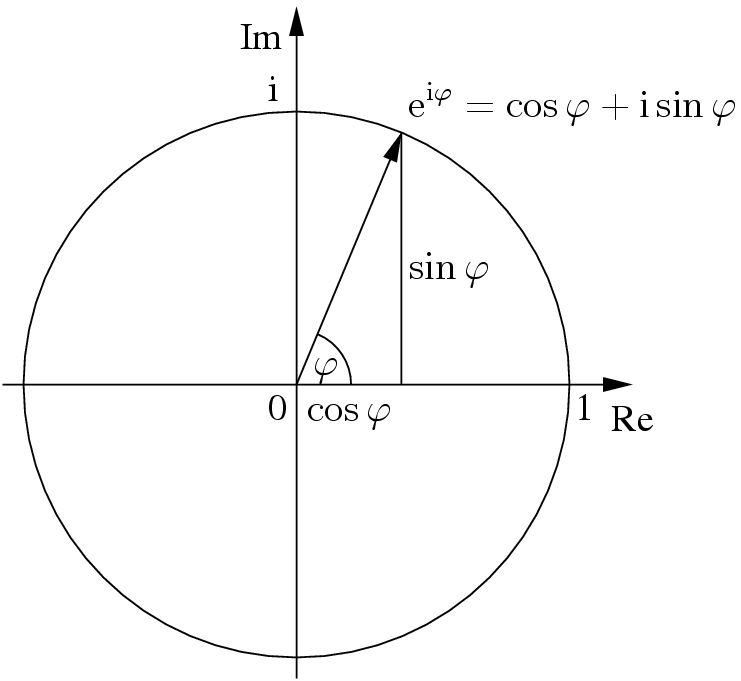
\includegraphics[scale=0.75]{eulerformel.jpg}
\end{center}

\subsection{Das Skalarprodukt von Funktionen und Orthonormalsysteme}
Des Weiteren spielen Orthonormalsysteme eine große Rolle, wenn man sich mit der Fourier Analyse beschäftigt. 
Allgemein lässt sich sagen, dass ein Orthonormalsystem eine Menge von Vektoren oder Funktionen, aus einem Vektorraum mit Skalarprodukt, 
sind, welche sowohl orthogonal zueinander, aber auch normiert zu sich selbst sind. 
Orthogonal sind sie, wenn das Skalarprodukt zweier unterschiedlicher Vektoren 0 ergibt und normiert, wenn das Skalarprodukt eines Vektors mit sich selbst 1 ergibt.
Für alle Vektoren $v_n$ im $\mathbb{R}^n$ muss also folgendes gelten, damit die Menge der Vektoren ein Orthonormalsystem bildet: 
$$\text{1. Orthogonalität: } \langle v_i, v_j\rangle = 0 \quad \forall \:i \neq j $$
$$\text{2. Normiertheit: } \langle v_i, v_j\rangle = \sum_{i=1}^{n}v_i^2 = \|v_i\|^2 = 1 \quad \text{mit} \: i = j$$
$$\left( \text{Skalarprodukt: } \langle v, w\rangle := \sum_{i = 1}^{n}v_i * w_i\right)$$
Hier sieht man auch, dass das Skalarprodukt eines Vektors mit sich selbst, das gleiche 
ist wie die quadrierte euklidische Norm des Vektors, wodurch der Begriff der Normiertheit 
anschaulicher wird. Wie schon erwähnt lassen sich diese Eigenschaften auch auf Funktionen anwenden. 
Hierfür definiert man die Normiertheit und die Orthogonalität auch, exakt gleich wie bei Vektoren, über das Skalarprodukt. Das Skalarprodukt für zwei Funktionen ist wie folgt definiert:
$$\langle v, w \rangle := \int_a^bv{(x)*w(x)dx} \quad \text{für} \: v,w : [a,b] \to \mathbb{R} $$
Falls eine Menge von Funktionen Orthogonalität und Normiertheit erfüllt, ist diese Menge auch ein Orthogonalsystem. 
Anschaulich kann man sich die Funktionen v(x) und w(x) noch als zwei Vektoren mit unendlich 
vielen Dimensionen vorstellen, wobei der x Wert angibt in welcher Dimension man sich befindet. 
Da das Skalarprodukt die jeweiligen Dimensionen von Vektoren multipliziert und diese 
schließlich aufsummiert, macht es Sinn, dass man bei Funktionen ähnlich vorgeht. 
So lässt sich also die Erweiterung der Summe zum Integral erklären.  Die Formel für die 
Norm von Funktionen $\left( \|f\| = \sqrt{\int_a^b{\vert f(x)\vert^2 dx}} \right)$ ergibt sich, wenn man das für Funktionen definierte Skalarprodukt 
ähnlich wie bei Vektoren auf die Funktion selbst anwendet. Im komplexen Fall wird das Skalarprodukt leicht angepasst, 
indem der zweite Faktor komplex konjugiert wird:
$$\langle v,w \rangle := \int_a^b{v(x)*\overline{w(x)}dx} \quad \text{für} \: v,w : [a,b] \to \mathbb{C}$$

\subsection{Die Fourierreihe}
Der erste große Schritt, um die Fourier Transformation herzuleiten, ist die Fourier Reihe. 
Eine Reihe selbst ist in der Mathematik ist ein Begriff für eine unendliche Summe von Termen. 
Die Fourier Reihe ist hierbei eine besondere Reihe. Ihr Sinn ist es periodische Funktionen 
mithilfe von Sinus- und Kosinustermen zu approximieren.  Joseph Fourier hat in seinem Werk 
„Théorie analytique de la chaleur“ schließlich auch beweisen, dass jede periodische Funktion 
auf diese Weise dargestellt werden kann. Die Approximation selbst geschieht durch 
trigonometrische Polynome, mit welchen man später die Fourierreihe einer Funktion bildet. 
Ein trigonometrisches Polynom ist hier eine Funktion der Form: 
$$p(x) = a_0 + \sum_{k=1}^n{a_k \cos(kx) + b_k \sin(kx)}  \quad a_k,b_k \in \mathbb{R}$$
Ziel ist es nun die Faktoren $a_k$ und $b_k$ in Abhängigkeit zur anzunähernden Funktion zu 
bestimmen. Denn durch die Zählervariable k, welche die Periodenlänge der Sinus- und 
Kosinusterme bestimmt, kann man durch die Faktoren $a_k$ und $b_k$ festlegen wie dominant 
die Anteile der Sinus und Kosinusterme, mit der jeweiligen Periodenlänge, in der zu 
approximierende Funktion sind. Um die Berechnung der Faktoren kompakter zu gestalten, 
kann man mit dem Zusammenhang $2\cos{x} = e^{ix} -e^{-ix}$ und $2i\sin{x} = e^{ix}+e^{-ix}$, 
einer Umstellung der Eulerformel, nun das trigonometrische Polynom zu dem komplexen 
trigonometrischen Polynom zusammenfassen: 
$$p(x) = \sum_{k=-n}^n{c_k \, e^{ikx}} \quad \text{für geeignete} \: c_k \in \mathbb{C}$$
Um jetzt den komplexen Faktor $c_k$, zunächst für $2\pi$ periodische Funktionen, 
zu berechnen, verwendet man ein Orthonormalsystem, welches aus den Funktionen $\varphi_n(x)$ besteht:
$$\phi_n(x):[-\pi,\pi] \to \mathbb{C}, \quad \phi_n(x) = \frac{1}{\sqrt{2\pi}} \, e^{inx} \quad \text{mit} \: n\in \mathbb{Z}$$
Dass die Menge an Funktionen $\phi_n$ ein Orthonormalsystem ist, habe 
ich im Anhang gezeigt (Beweis A. 1). Um endlich $c_k$ zu berechnen, setzt man zunächst 
die zu approximierende Funktion $f$, mit der Periodizität $2\pi$, mit dem 
trigonometrischen Polynom gleich und schränkt sie zudem ein: 
$$f:[-\pi,\pi]\to \mathbb{C},\quad f(x) = \sqrt{2\pi} * \sum_{k = -n}^n{c_k\phi_k(x)} $$
Anschließend bildet man das Skalarprodukt von $f$ und $\phi_m$, was möglich ist, da 
$f$ auf der Definitionsbereich von $f$ und $\phi_m$ gleich ist. 
$$\langle f, \phi_m \rangle = \int_{-\pi}^\pi {f(x) \overline{\phi_m(x)}dx} = \int_{-\pi}^\pi{\sqrt{2\pi}\sum_{k = -n}^n{c_k\phi_k(x)\overline{\phi_m(x)}}dx}$$
Da Integral und Summe beide linear sind, darf man die Summe mit dem Integral vertauschen. 
Zudem hängt $c_k$ nicht von $x$ ab, wodurch der Faktor $c_k$ für das Integral eine Konstante ist. 
Nach einer Abwandlung des Distributivgesetzes darf er somit herausgezogen werden. Man erhält 
also diesen Ausdruck: 
$$\int_{-\pi}^\pi{f(x)\overline{\phi_m(x)} dx} = \sqrt{2\pi}\sum_{k=-n}^{n}{c_k\int_{-\pi}^\pi{\phi_k(x) \overline{\phi_m(x)} dx}}$$
Aufgrund dessen, dass die Menge der Funktionen $\phi_m$ ein Orthonormalsystem ist, ist jeder Summand, außer $k = m$, 0. Durch die Normiertheit des Orthonormalsystems bleibt übrig:
$$c_m = \frac{1}{\sqrt{2\pi}}\int_{-\pi}^\pi{f(x)\overline{\phi_m(x)}dx} = \frac{1}{2\pi}\int_{-\pi}^\pi{f(x)e^{imx}dx}$$ 

Jetzt ist es möglich mit dieser Formel und dem komplexen trigonometrischem Polynom eine 
$2\pi$ periodische Funktion zu approximieren. Jedoch wäre es hilfreich, wenn dies für alle 
Perioden möglich wäre. Um auch Funktionen mit einer Periodizität von $2L$ annähern zu können, 
muss man den Faktor $c_k$ und das komplexe trigonometrische Polynom auf einer Periodizität von $2L$ ausweiten. 
Damit das trigonometrische Polynom $2L$ periodisch wird muss folgendes gelten: 
$$e^{i\omega x} = e^{i\omega(x+2L)}$$
$\omega$ gilt es dabei herauszufinden, damit das trigonometrische Polynom $2L$ periodisch wird:
$$e^{i\omega x} = e^{i\omega(x+2L)} \Leftrightarrow e^{i\omega 2L} = 1 \Leftrightarrow \omega 2L = 2\pi k \Leftrightarrow \omega_k = \frac{k\pi}{L}$$
Das neue trigonometrische Polynom sieht also so aus:
$$\sum_{k=-n}^n{c_k e^{i\omega_kx}} \Leftrightarrow \sum_{k=-n}^n{c_k e^{i\frac{k\pi}{L}x}}$$
Um $c_k$ zu berechen, nimmt man sich eine $2L$ periodische Funktion $f$ und definiert sich eine $2\pi$ periodische 
Hilfsfunktion $g$ in Abhängigkeit von $f$ wie folgt:
$$g(t) := f\left(\frac{L}{\pi}t\right) $$
Da $g$ eine $2\pi$ periodische Funktion ist, kann man mit der hergeleiteten Formel $c_k$ 
von $g$ berechnen. Um die Formel für $2L$ periodische Funktionen zu erhalten, ist das 
Ziel die Formel über $g$ auf $f$ auszuweiten. Das funktioniert über die Substitutionsregel 
bei Integralen. Um sie anzuwenden, führen wir die Ableitung der inneren Funktion von $f$, 
also $\frac{L}{\pi}$ in Form einer $1$ ein und erhalten die Formel für $c_k$, für die 
Periodizität $2L$: 
$$c_k = \frac{1}{2\pi} \int_{-\pi}^\pi{g(t)e^{-ikt}dt} \Leftrightarrow c_k = \frac{1}{2\pi}*\frac{\pi}{L} \int_{-\pi}^{\pi}{\frac{L}{\pi}f\left(\frac{L}{\pi}t\right)e^{-i\omega_kt} dt}$$
Wendet man jetzt die Substitutionsregel an, erhält man: 
$$c_k = \frac{1}{2L}\int_{-L}^{L}{f(x)e^{-i\omega_kx}dx} = \frac{1}{2L}\int_{-L}^{L}{f(x)e^{-i\frac{k\pi}{L}x}dx}$$

\subsection{Von der Fourierreihe zur Fouriertranformation}
Die Fourierreihe erlaubt es uns, periodische Signale als Summe von Sinus- und Kosinusfunktionen oder komplexen Exponentialfunktionen darzustellen. Doch viele Signale in der Praxis sind nicht-periodisch. Um auch diese Signale in ihre Frequenzanteile zerlegen zu können, verallgemeinern wir das Konzept der Fourierreihe zur Fouriertransformation. Mit der Fouriertransformation werden wir so eine Funktion erhalten, welche uns sagen wird wie groß der Anteil einer Frequenz oder Periodenlänge in einem Signal ist. Dazu nehmen wir die Fourierreihe einer Funktion $f$ mit der Periode $2L$ und der Frequenz $\omega_k$: 
$$f(x) = \sum_{k = -\infty}^{\infty}{c_k e^{i\omega_k x} }, \quad c_k = \frac{1}{2L}\int_{-L}^L{f(x) e^{-i\omega_k x} dx}$$
Dazu definieren wir eine Hilfsfunktion $F(\xi)$: 
$$F:\mathbb{R} \to \mathbb{C}, \quad F(\xi) = \int_{-L}^{L}{f(x) e^{-i \xi x} dx}$$
damit gilt
$$ c_k = \frac{1}{2L} F(\omega_k)$$
Setzt man den neu gewonnen Ausdruck für $c_k$ in die Fourierreihe ein, so erhält man 
$$ f(x) = \sum_{n = -\infty}^{\infty}{F(\omega) e^{i\omega x}}$$
Anschließend bildet man $\Delta \omega$ aus $\omega_k$:
$$\omega_k = k \frac{\pi}{L} \Rightarrow \Delta \omega = \frac{\pi}{L} \Rightarrow \frac{1}{2L} = \frac{\Delta \omega} {2\pi}$$
Und setzt die Gleichung auch in die Fourierreihe ein: 
$$\frac{1}{2\pi} \sum_{k=-\infty}^{\infty}{F(\omega_k) e^{i \omega_k x} \Delta \omega}$$
Dies ist eine Riemann Summe. Lässt man nun $L \to \infty$ laufen, erhält man ein Integral, welches die inverse Fouriertransformation ist:
$$\lim_{L\to\infty} {\frac{1}{2\pi}\sum_{n = -\infty}^\infty{F(\omega_k) e^{i \omega_k x}\Delta \omega}} = \frac {1}{2\pi} \int_{-\infty}^{\infty}{F(\omega)e^{i \omega x} d\omega}$$
Die Funktion $F(\omega)$ selbst ist die Fouriertransformation von $f$:
$$F(\omega) = \int_{-\infty}^{\infty}{f(x) e^{-i\omega x} dx}$$

Man kann das Integral in der Fouriertransformation am besten verstehen, wenn man es 
als eine Art Durchschnitt betrachtet. Ähnlich wie beim Berechnen eines Mittelwerts 
summiert das Integral nicht nur eine endliche Anzahl von Werten auf, sondern unendlich viele, 
unendlich kleine Beiträge von $f(x)$. Im Integral steht dabei das Produkt $f(x) \cdot e^{-i\omega x}$.
Dieses Produkt misst, wie stark die Frequenz $\omega$ in $f(x)$ enthalten ist:
\begin{itemize}
    \item Ist der Anteil der Frequenz $\omega$ in $f(x)$ hoch, dann verstärkt $e^{i\omega_kx}$ den Wert der Funktion $f(x)$
    im Integral konstruktiv und $F(\omega)$ wird groß.
    \item Enthält $f(x)$ diese Frequenz nicht, heben sich die positiven und negativen Anteile 
    im Integral weitgehend auf und $F(\omega)$ wird klein.
\end{itemize}
So zeigt die Fouriertransformation, wie groß der Anteil jeder einzelnen Frequenz $\omega$ 
in der Funktion $f$ ist.

\subsection{Die Foureirtransformation in der Praxis: Die DFT}
In der Praxis arbeitet man selten mit kontinuierlichen Funktionen, sondern mit diskreten Messwerten, zum Beispiel bei Audiosignalen oder digitalen Bildern. Um diese Signale in ihre Frequenzanteile zu zerlegen, verwendet man die diskrete Fouriertransformation (DFT).
Formell lässt sich die DFT für eine endliche Folge von N Messwerten
$$x_0, x_1,..., x_{N-1}$$
durch die folgende Formel darstellen:
$$X_k = \sum_{n = 0}^{N-1}{x_n e^{-i2\pi \frac{kn}{N}}} \quad \text{mit } k\in[0, N-1]$$
Anzumerken ist aber noch, dass es eine Besonderheit gibt. Wenn das Eingangssignal reell ist, 
liefert die DFT zwar N Koeffizienten, jedoch sind die Frequenzen oberhalb von N/2 wegen des 
Nyquist-Theorems lediglich Spiegelungen der tieferen Frequenzen und enthalten keine neuen 
Informationen. Warum das so ist, werde ich hier nicht näher eingehen. Wie man die Formel für 
die DFT herleitet, erkläre ich im nächsten Kapitel.

\subsection{Die Foureirtransformation in der Praxis: Die FFT}

\section{Fourier-Reihe}
\subsection{Herleitung der Reihe}
\subsection{Berechnung der Koeffizienten}
\subsection{Eigenschaften und Konvergenz}

\section{Von der Reihe zur Fourier-Transformation}
\subsection{Übergang zum Integral}
\subsection{Fourier-Transformation und inverse Transformation}
\subsection{Eigenschaften}
Linearität, Verschiebung, Faltung.

\section{Diskrete Fourier-Transformation (DFT)}
\subsection{Definition und Motivation}
\subsection{Herleitung aus der Fourier-Transformation}
Eigene Herleitung
\subsection{Beweise für die Korrektheit}
\subsection{FFT als effiziente Berechnung}

\section{Eigene Beiträge}
\subsection{Eigene Herleitung der DFT}
\subsection{Beweise}
\subsection{Eigener FFT-Algorithmus in Python}
\subsection{Audio-Programm zur Echtzeit-Visualisierung}

\begin{figure}[h!]
\centering
\begin{tikzpicture}
    \begin{axis}[
    width=\textwidth,
    height=8cm,
    xlabel={Zeit [s]},
    ylabel={Zeit [s]},
    grid=major,
    major grid style={gray!30},
    legend style={at={(0.5,-0.2)}, anchor=north, legend columns=2, font=\small},
    label style={font=\large},
    tick label style={font=\small},
    line width=1pt,
    no markers,
    cycle list={
        {blue},
        {red},
        {brown},
        {black},
        {teal}
        }
        ]
        
        \addplot table[x index=1, y expr=\thisrowno{2}/1000] {fft_bench5.dat};
        \addlegendentry{Rekursive FFT}
        
        \addplot table[x index=1, y expr=\thisrowno{3}/1000] {fft_bench5.dat};
        \addlegendentry{Iterative FFT}
        
        \addplot table[x index=1, y expr=\thisrowno{4}/1000] {fft_bench5.dat};
        \addlegendentry{Iterative FFT auf GPU}
        
        \addplot table[x index=1, y expr=\thisrowno{5}/1000] {fft_bench5.dat};
        \addlegendentry{cuFFT-Bibliothek (GPU)}
        
        \addplot table[x index=1, y expr=\thisrowno{6}/1000] {fft_bench5.dat};
        \addlegendentry{FFTW-Bibliothek (CPU)}
        
        
    \end{axis}
\end{tikzpicture}
\caption{Vergleich der FFT-Methoden anhand der Benchmarks.}
\end{figure}

\begin{figure}[h!]
    \centering
    \begin{tikzpicture}
        \begin{axis}[
            width=\textwidth,
            height=8cm,
            xlabel={Zeit [ms]},
            ylabel={Zeit [ms]},
            grid=major,
            major grid style={gray!30},
            legend style={at={(0.5,-0.2)}, anchor=north, legend columns=2, font=\small},
            label style={font=\large},
            tick label style={font=\small},
            line width=1pt,
            no markers,
            cycle list={
                {blue},
                {red},
                {brown},
                {black},
                {teal}
                }
                ]
                
                \addplot table[x expr=\thisrowno{1}*1000, y index=2] {fft_bench_small.dat};
                \addlegendentry{Rekursive FFT}
                
                \addplot table[x expr=\thisrowno{1}*1000, y index=3] {fft_bench_small.dat};
                \addlegendentry{Iterative FFT}
                
                \addplot table[x expr=\thisrowno{1}*1000, y index=4] {fft_bench_small.dat};
                \addlegendentry{Iterative FFT auf GPU}
                
            \end{axis}
        \end{tikzpicture}
        \caption{Vergleich der FFT-Methoden für die zweite Messreihe.}
    \end{figure}
    
    \begin{figure}[h!]
        \centering
        \begin{tikzpicture}
            \begin{axis}[
                width=\textwidth,
                height=8cm,
                xlabel={Zeit [min]},
                ylabel={Zeit [s]},
                grid=major,
                major grid style={gray!30},
                legend style={at={(0.5,-0.2)}, anchor=north, legend columns=2, font=\small},
                label style={font=\large},
                tick label style={font=\small},
                line width=1pt,
                no markers,
                cycle list={
                    {black},
                    {teal}
                    }
                    ]
                    
                    \addplot table[x expr=\thisrowno{1}/60, y expr=\thisrowno{2}/1000] {fft_bench_big.dat};
                    \addlegendentry{cuFFT-Bibliothek (GPU)}
                    
                    \addplot table[x expr=\thisrowno{1}/60, y expr=\thisrowno{3}/1000] {fft_bench_big.dat};
                    \addlegendentry{FFTW-Bibliothek (CPU)}
                    
                \end{axis}
            \end{tikzpicture}
            \caption{Vergleich der FFT-Methoden für die zweite Messreihe.}
        \end{figure}
        
        \subsection{Bildverarbeitung: Moiré-Muster entfernen mit 2D-FFT}
        
        \section{Anwendungen}
        \subsection{Audio}
        Echtzeitaufnahme und Visualisierung, Tonhöhenerkennung oder Noise Cancelling, Ergebnisse.
        \subsection{Bild}
        Röntgenbild und Moiré-Filterung, Ergebnisse.
        
        \section{Anhang}
        \begin{theorem}\label{thm:orthonorm}
            Die Menge $\{\phi_n(x)\}_{n\in\mathbb{Z}}$ mit $\phi_n:[-\pi, \pi] \to \mathbb{C}, \\ \phi_n(x) = \frac{1}{\sqrt{2\pi}}e^{inx}$ bildet ein Orthonormalsystem.
        \end{theorem}
        
        \begin{proof}
            Ich zeige die Orthonormalität in zwei Schritten: 
            
            \textbf{1. Orthogonalität:}  
            Für $m \neq n$ gilt
            $$\langle \phi_n, \phi_m \rangle = \int_{-\pi}^{\pi}{\phi_n(x) \overline{\phi_m(x)}} = \frac{1}{2\pi}\int_{-\pi}^\pi{e^{i(n-m)x}dx}$$
            
            Jetzt definiere ich $l := n-m$
            \[\frac{1}{2\pi}\int_{-\pi}^\pi{e^{i(n-m)x}dx} = \frac{1}{2\pi}\int_{-\pi}^\pi{\cos(lx) + i \sin (lx)} dx\] 
            
            \[= \frac{1}{2\pi l}\left(\int_{-\pi}^\pi{\cos (lx) dx} + i\int_{-\pi}^\pi{ \sin (lx) dx} \right)  = \frac{1}{2\pi l} \left(\sin(lx)\big|_{-l\pi}^{l\pi} - i\cos(lx)\big|_{-l\pi}^{l\pi} \right)\]
            
            \[= \frac{1}{2\pi l} \cdot \left(\sin(l^2\pi) - \sin(-l^2\pi) - i\left(\cos(l^2\pi) - \cos(-l^2\pi)\right)\right) \]
            
            Da $l\in \mathbb{Z}$ ist $l^2 \in \mathbb{Z}$. Ein ganzzahliges Vielfaches von $\pi$
            eingesetzt im Sinus ist zudem immer 0. Denn der Sinus ist eine $2\pi$ periodische Funktion, und da
            sowohl $\sin(0) = 0$, als auch $\sin (\pi) = 0$ ist, ist jedes ganzzahliges Vielfaches von $\pi$ eingesetzt 
            im Sinus 0. Hinzu kommt, dass der Kosinus Achsensymmetrisch bezüglich der Y-Achse ist, also gilt:
            $\cos (x) =  \cos (-x)$. Daraus folgt:
            \[= \frac{1}{2\pi l} \cdot (0 - 0 - i\cdot(\cos(l\pi) - \cos(l\pi))) = \frac{1}{2\pi l} \cdot 0 = 0\]
            
            
            \textbf{2. Normierung:}  
            Für $m = n$ gilt
            
            \[\langle \phi_n, \phi_m \rangle = \int_{-\pi}^{\pi} \phi_n(x) \overline{\phi_n(x)} \, dx = \frac{1}{2\pi} \int_{-\pi}^{\pi} e^{i(n -n) x}\, dx = \frac{1}{2\pi} \int_{-\pi}^{\pi} e^{i\cdot0} \, dx\]
            
            \[= \frac{1}{2\pi} \int_{-\pi}^{\pi} 1 \, dx = \frac{1}{2\pi} \cdot x \Big|_{-\pi}^{\pi} = \frac{1}{2\pi} \cdot (\pi-(-\pi)) = 1\]
            
            Damit ist gezeigt, dass $\{\phi_n(x)\}_{n\in\mathbb{Z}}$ ein Orthonormalsystem bildet.
        \end{proof}
\subsection{Stärken und Grenzen}
\subsection{Bedeutung im größeren Kontext}
        

\begin{figure}[h!]
\centering
\begin{tikzpicture}[>=stealth]

% Achsen
\draw[->] (-0.5,0) -- (15.5,0) node[right] {$n$};
\draw[->] (0,-2.5) -- (0,2.5) node[above] {$f(n)$};

% Winkel pro Einheit (in Grad) sodass 1.5 Perioden auf [0,14] liegen
\pgfmathsetmacro{\degPerUnit}{180*3/14} % = 38.5714286...

% Diskrete Punkte f(n) (aus der Sinusfunktion)
\foreach \x in {0,...,14} {
    \pgfmathsetmacro{\yy}{2*sin(\degPerUnit*\x)} % sin erwartet hier Grad
    \fill[red] (\x,\yy) circle (2pt);
    \node[red, above, font=\scriptsize] at (\x,\yy) {$f(\pgfmathprintnumber{\x})$};
    \draw[dashed, gray!60] (\x,0) -- (\x,\yy);
}

% Linien zwischen Punkten (Stückweise verbunden)
\draw[thick, blue] (0,{2*sin(0)})
\foreach \x in {1,...,14} {
   -- (\x,{2*sin(\degPerUnit*\x)})
};

% Trapezflächen (je zwei aufeinanderfolgende Punkte)
\foreach \i in {0,...,13} {
    \pgfmathsetmacro{\yone}{2*sin(\degPerUnit*\i)}
    \pgfmathsetmacro{\ytwo}{2*sin(\degPerUnit*(\i+1))}
    \pgfmathsetmacro{\xnext}{\i+1}
    \fill[blue!20, opacity=0.5] (\i,0) -- (\i,\yone) -- (\xnext,\ytwo) -- (\xnext,0) -- cycle;
}

% (Optional) kontinuierliche Referenz-Sinuskurve mit gleicher Frequenz
\draw[domain=0:14, smooth, samples=300, thin, red!70] plot(\x,{2*sin(\degPerUnit*\x)});

% Beschriftung Trapezformel
\node at (9,-2.3) {\footnotesize Fläche Trapez: $A = \tfrac{1}{2} (x_{n+1}-x_n)\,(f(n)+f(n+1))$};

\end{tikzpicture}
\caption{Diskrete Werte einer Sinuskurve (Amplitude 2) — 1{,}5 Perioden über 0 bis 14.}
\end{figure}

                
                
\section{Fazit und Ausblick}
\subsection{Zusammenfassung der Ergebnisse}
\subsection{Ausblick: Erweiterungen und Anwendungen}
                
\end{document}
                